%; whizzy chapter -dvi
% -initex iniptex -latex platex -format platex -bibtex jbibtex -fmt fmt
% 以上 whizzytex を使用する場合の設定。

%     Tokyo Debian Meeting resources
%     Copyright (C) 2012 Junichi Uekawa
%     Copyright (C) 2011, 2015, 2020 Nobuhiro Iwamatsu

%     This program is free software; you can redistribute it and/or modify
%     it under the terms of the GNU General Public License as published by
%     the Free Software Foundation; either version 2 of the License, or
%     (at your option) any later version.

%     This program is distributed in the hope that it will be useful,
%     but WITHOUT ANY WARRANTY; without even the implied warranty of
%     MERCHANTABILITY or FITNESS FOR A PARTICULAR PURPOSE.  See the
%     GNU General Public License for more details.

%     You should have received a copy of the GNU General Public License
%     along with this program; if not, write to the Free Software
%     Foundation, Inc., 51 Franklin St, Fifth Floor, Boston, MA  02110-1301 USA

%  preview (shell-command (concat "evince " (replace-regexp-in-string "tex$" "pdf"(buffer-file-name)) "&"))

%%ここからヘッダ開始。

\documentclass[mingoth,a4paper]{jsarticle}
\usepackage{monthlyreport}
% 日付を定義する、毎月変わります。
\newcommand{\debmtgyear}{2020}
\newcommand{\debmtgmonth}{5}
\newcommand{\debmtgdate}{16}
% started from zero:
% (let ((year 2013) (month 7)) (+ (* (- year 2005) 12) month -1))
\newcommand{\debmtgnumber}{185}

% Needed to import pandoc-generated LaTeX documents.
% See https://stackoverflow.com/questions/40438037/tightlist-error-using-pandoc-with-markdown
\providecommand{\tightlist}{%
  \setlength{\itemsep}{0pt}\setlength{\parskip}{0pt}}

% tikz picture の為のマクロ設定
\usepackage[dvipdfmx]{graphicx}
\usepackage{tikz}

\begin{document}

\begin{titlepage}
\thispagestyle{empty}
% タイトルページ:編集必要な部分は最初のマクロに飛ばすこと

\vspace*{-2cm}
第\debmtgnumber{}回 東京エリア Debian 勉強会資料\\
\hspace*{-2cm}

\includegraphics{image2012-natsu/dotdeb.pdf}\\
\hfill{}\debmtgyear{}年\debmtgmonth{}月\debmtgdate{}日

% ここはアップデートすること
% 全角文字にしないとフォントのサイズが合わないので注意
\rotatebox{10}{\fontsize{30}{30} {\gt aptly特集}}\\

\vspace*{-2cm}
\hfill{}
\includegraphics[height=6cm]{image200502/openlogo-nd.eps}
\end{titlepage}

\newpage

\begin{minipage}[b]{0.2\hsize}
 \definecolor{titleback}{gray}{0.9}
 \colorbox{titleback}{\rotatebox{90}{\fontsize{80}{80} {\gt デビアン勉強会} }}
\end{minipage}
\begin{minipage}[b]{0.8\hsize}
\hrule
\vspace{2mm}
\hrule
\begin{multicols}{2}
\tableofcontents
\end{multicols}
\vspace{2mm}
\hrule
\end{minipage}

\dancersection{最近のDebian関連のミーティング報告}{杉本 典充}

\subsection{2020年4月度 東京エリア・関西合同Debian勉強会}

2020年4月18日(土)に東京エリアDebian勉強会と関西Debian勉強会の合同でオンラインによるDebian勉強会を開催しました。参加者は35名でした。セミナー発表を2つ行いました。


セミナー「Wireguard 実践入門」という表題で西山和広さんが発表しました。WireguardはVPN接続するアプリケーションであり、サーバとクライアントをスター型で接続する構成の他、メッシュ型の接続も可能との説明でした。linux-5.6より古いカーネルの場合はカーネルモジュールをDKMSでビルドして利用し、linux-5.6以降ではカーネルにマージされているなど最新の動向の説明がありました。また、質疑応答ではOpenVPNと対比する質問がありました。


セミナー「Jitsiを使ったビデオ会議サーバの作り方」という表題で杉本典充さんが発表しました。2020年3月に開催したDebian勉強会はインターネットを用いたビデオ会議形式で開催しており、そのときに利用したアプリケーションであるJitsi(ジッチー)を説明しました。JitsiをGCPのサーバにインストールして使えるようにする手順の説明、設定のカスタマイズ方法の紹介、2020年3月に開催したDebian勉強会のときのサーバのCPU利用率とトラフィックグラフを紹介しました。


\dancersection{事前課題}{杉本 典充}

今回の事前課題は以下です。

\begin{enumerate}
\item aptly はご存じですか
\end{enumerate}

%この課題に対して提出いただいた内容は以下です。

\begin{multicols}{2}
{\small
\begin{prework}{ dictoss }
  \begin{enumerate}
  \item $BCN$i$J$$(B
  \end{enumerate}
\end{prework}

\begin{prework}{ yy\_y\_ja\_jp }
  \begin{enumerate}
  \item $BCN$i$J$$(B
  \end{enumerate}
\end{prework}

\begin{prework}{ uwabami }
  \begin{enumerate}
  \item $BCN$C$F$$$k$,!";H$C$?$3$H$O$J$$(B
  \end{enumerate}
\end{prework}

\begin{prework}{ yosuke\_san }
  \begin{enumerate}
  \item $BCN$i$J$$(B
  \end{enumerate}
\end{prework}

\begin{prework}{ $B$"(B (cpa119) }
  \begin{enumerate}
  \item $BCN$i$J$$(B
  \end{enumerate}
\end{prework}

\begin{prework}{ MasanoriYoshida }
  \begin{enumerate}
  \item $BCN$i$J$$(B
  \end{enumerate}
\end{prework}

\begin{prework}{ NOKUBI Takatsugu (knok) }
  \begin{enumerate}
  \item $BCN$i$J$$(B
  \end{enumerate}
\end{prework}

\begin{prework}{ su\_do }
  \begin{enumerate}
  \item $BCN$i$J$$(B
  \end{enumerate}
\end{prework}

\begin{prework}{ TANIGUCHI Takaki (takaki\_t) }
  \begin{enumerate}
  \item $BCN$i$J$$(B
  \end{enumerate}
\end{prework}

\begin{prework}{ noncatalyst }
  \begin{enumerate}
  \item $BCN$i$J$$(B
  \end{enumerate}
\end{prework}

\begin{prework}{ kozo2 }
  \begin{enumerate}
  \item $BCN$i$J$$(B
  \end{enumerate}
\end{prework}

\begin{prework}{ matoken }
  \begin{enumerate}
  \item $BCN$C$F$$$k$,!";H$C$?$3$H$O$J$$(B
  \end{enumerate}
\end{prework}

\begin{prework}{ $B%W%i%$%K%s%0!!%N%k%Y%k%H(B (norbu) }
  \begin{enumerate}
  \item $B;H$C$?$3$H$,$"$k(B
  \end{enumerate}
\end{prework}

\begin{prework}{ Katsuki Kobayashi (rarewin) }
  \begin{enumerate}
  \item $BCN$i$J$$(B
  \end{enumerate}
\end{prework}

\begin{prework}{ koedoyoshida }
  \begin{enumerate}
  \item $BCN$i$J$$(B
  \end{enumerate}
\end{prework}

\begin{prework}{ $B1]??<#(B (enoki) }
  \begin{enumerate}
  \item $BCN$i$J$$(B
  \end{enumerate}
\end{prework}

\begin{prework}{ daromart }
  \begin{enumerate}
  \item $BCN$C$F$$$k$,!";H$C$?$3$H$O$J$$(B
  \end{enumerate}
\end{prework}

\begin{prework}{ Incognito (cyberconn) }
  \begin{enumerate}
  \item $BCN$i$J$$(B
  \end{enumerate}
\end{prework}

\begin{prework}{ ipv6waterstar }
  \begin{enumerate}
  \item $BCN$C$F$$$k$,!";H$C$?$3$H$O$J$$(B
  \end{enumerate}
\end{prework}

\begin{prework}{ Kazuhiro NISHIYAMA (znz) }
  \begin{enumerate}
  \item $BCN$i$J$$(B
  \end{enumerate}
\end{prework}

\begin{prework}{ Kouhei Maeda (mkouhei) }
  \begin{enumerate}
  \item $BCN$C$F$$$k$,!";H$C$?$3$H$O$J$$(B
  \end{enumerate}
\end{prework}

}
\end{multicols}

%\dancersection{Debian Trivia Quiz}{username}
%
%Debianの昨今の話題についてのQuizです。
%
%今回の出題範囲は\url{debian-devel-announce@lists.debian.org} や \url{debian-news@lists.debian.org}などに投稿された内容からです。
%
%\begin{multicols}{2}
%%; whizzy-master ../debianmeetingresume201211.tex
% $B0J>e$N@_Dj$r$7$F$$$k$?$a!"$3$N%U%!%$%k$G(B M-x whizzytex $B$9$k$H!"(Bwhizzytex$B$,MxMQ$G$-$^$9!#(B
%

\santaku
{DebConf13 $B$N3+:ECO$H3+:EF|$O!)(B}
{$BF|K\!"El5~ET(B 6$B7n(B20$BF|(B}
{$B%K%+%i%0%"(B $B%^%J%0%"(B 7$B7n(B8-14$BF|(B}
{$B%9%$%9!"%t%)!<%^%k%-%e(B 8$B7n(B11-18$BF|(B}
{3}
{$B%K%+%i%0%"$O(BDebConf12$B$N3+:ECO$G$9!#(B
DebConf13$B$O%9%$%9$N%-%c%s%WCO$G3+:E$G$9!#(B
6/20$B$O3'$5$sM=Dj$r6u$1$F$*$-$^$7$g$&!#(B}

\santaku
{$B@$3&$N(BWeb$B%5!<%P$G:G$b?M5$$N$"$k(BLinux $B%G%#%9%H%j%S%e!<%7%g%s(B(W3Techs$BD4$Y(B)$B$O!)(B}
{CentOS}
{Debian}
{Ubuntu}
{B}
{\url{http://w3techs.com/technologies/history_details/os-linux}$B$K7k2L$N%0%i%U$,$"$j$^$9!#(B
$B8=:_(B Linux $B$r;HMQ$7$F$$$k(B web $B%5!<%P$N(B 32.9\% $B$,(B Debian $B$rMxMQ$7$F$*$j!"$=$N3d9g$O8=:_$bA}2C$rB3$1$F$$$k$=$&$G$9!#(B}

\santaku
{Debian $B%+!<%M%k%A!<%`$N%a%s%P!<$G$"$j!"(Bkernel.org $B$N(B 3.2.y $B0BDjHG7ONs$N%a%s%F%J$G$b$"$k(B Ben Hutchings $B$5$s$,<!4|(B Debian $B0BDjHG$H0l=o$K=P2Y$5$l$k(B Linux $B%+!<%M%k$K(B (3.2 $B7ONs$N(B mainline $B$K$OL5$$(B) $BDI2C5!G=$,Ek:\$5$l$kM=Dj$G$"$k$H=R$Y$F$$$^$9!#(B
$BB?$/$NDI2CE@$NCf$K4^$^$l$J$$$b$N$O2?!)(B}
{PREEMPT\_RT}
{Hyper-V guest drivers$B$N6/2=(B}
{ARM64/AArch64$B%"!<%-%F%/%A%c%5%]!<%H(B}
{C}
{Hyper-V guest drivers$B$O(Bmainline kernel$B$G(B3.2$B$K$b4^$^$l$F$$$^$9$,!"$h$j2~A1$5$l$?(B3.4$B$+$i$N=$@5$,F3F~$5$l$^$9!#(B
PREEMPT\_RT$B$O%O!<%I%j%"%k%?%$%`$r<B8=$9$k$?$a$N(BPatch$B!"(B
linux-image-rt-amd64 , linux-image-rt-686-pae $B$N(Bmetapackage$B$G;HMQ$G$-$^$9!#(B
$B?7$7$$(BARM 64$B%S%C%H%"!<%-%F%/%A%c%5%]!<%H$O(Bmainline kernel 3.7$B$+$i(B}

\santaku
{Wookey$B$5$s$,%"%J%&%s%9$7$?(Balpha$BHG$N(BDebian port arm64 image$B$O!)(B}
{Debian/Ubuntu port image}
{Debian/KFreeBSD port image}
{Debian/GnuHurd port image}
{A}
{self-bootstrapp(non x86)$BBP1~$H$N$3$H$G$9!#(B\url{http://wiki.debian.org/Arm64Port}$B$G%9%F!<%?%9$,3NG'$G$-$^$9!#(B}

\santaku
{700,000$BHVL\$N%P%0$,Js9p$5$l$?F|$rEv$F$k(B700000thBugContest$B$N7k2L$,=P$^$7$?!#$=$NM=A[F|$HJs9pF|$O!)(B}
{2012/12/12$B$rM=A[$7$?(BDavidPrevot}
{$BM=A[F|(B:2013/02/04$B!"Js9pF|(B:2013/02/14}
{$BM=A[F|(B:2013/02/07$B!"Js9pF|(B:2013/02/14}
{$BM=A[F|(B:2013/02/14$B!"Js9pF|(B:2013/02/07}
{C}
{$B:G$b6a$$(B2013/02/14$B$rM=A[$7$?(BChristian Perrier$B$5$s$,Ev$F$^$7$?!#7k2L$O(B\url{http://wiki.debian.org/700000thBugContest}$B$G8x3+$5$l$F$$$^$9!#(B
$B$^$?!"(B800,000/1,000,000$BHVL\$N%P%0$,Js9p$5$l$kF|$rEv$F$k%3%s%F%9%H(B\url{http://wiki.debian.org/800000thBugContest}$B$b3+:E$5$l$F$$$^$9!#(B}

\santaku
{master.debian.org$B$,?7$7$$5!3#$K0\9T$5$l$^$7$?!#$3$l$O2?$N%5!<%P$G$7$g$&$+(B $B!)(B}
{@debian.org$B$N%a!<%k%5!<%P(B}
{$B%Q%C%1!<%8$N%^%9%?!<%5!<%P(B}
{$B%Q%C%1!<%8$N%9%]%s%5!<(B(mentor)$B$rC5$9%5!<%P(B}
{A}
{$B8E$$%5!<%P$O%G%#%9%/>c32Ey$,$"$C$?$N$G!"<wL?$HH=CG$5$l!"%G!<%?$,B;<:$9$kA0$K?7$7$$%5!<%P$K0\9T$5$l$^$7$?!#(Bftp-master.debian.org$B$O(BDebian$B$N(B official package $B%j%]%8%H%j$G$9!#%Q%C%1!<%8$N%9%]%s%5!<(B(mentor)$B$rC5$9$N$O(Bmentors.debian.net$B!#(B }

\santaku
{pbuilder$B$K(Bclang support$B$,DI2C$5$l$^$7$?!#C/$,=q$$$?%Q%C%A$G$7$g$&$+!)(B}
{Sylvestre Ledru}
{Junichi Uekawa}
{Hideki Yamane}
{C}
{Debian$B$N(BClang$B%5%]!<%H$OCe!9$H?J$s$G$$$^$9!#(B}

\santaku
{DPN - 2013$BG/(B3$B7n(B4$BF|9f$K<h$j>e$2$i$l$?F|K\$N%$%Y%s%H$O(B}
{Open Source Conference 2013 Tokyo/Spring}
{Open Source Conference 2013 Hamamatu}
{Open Source Conference 2013 Tokushima}
{A}
{\url{http://henrich-on-debian.blogspot.jp/2013/02/open-source-conference-2013-tokyospring.html} $B>\:Y$O8e$[$I!#(B}


%\end{multicols}


% % (query-replace-regexp "<.*?>" "")
% % (query-replace-regexp "^[    ]\+" "")

\dancersection{aptly}{岩松 信洋}
%-------------------------------------------------------------------------------

Debian パッケージリポジトリのミラー作成、独自のパッケージリポジトリ作成などを
サポートするツール、aptlyについて説明します。

\subsection{aptly とは}

aptly (\url{https://www.aptly.info/}) は Debian パッケージリポジトリの作成・管理するツールの一つです。
パッケージリポジトリの作成やミラーリングを行うツールとして、dpkg-dev、apt-ftparchive、reprepro、archvsync などがありますが、
これらは機能が限定的であり、いくつかのツールを組み合わせて使うことがほとんどです。aptly はこれらをまとめた
機能を提供しています。

\begin{itemize}
\item パッケージリポジトリのフルミラーリングおよびフィルターミラーリング(アーキテクチャー、コンポーネント、パッケージ)
\item パッケージリポジトリのスナップショット作成
\item  パッケージリポジトリの更新、マージ、リリース
\item パッケージリポジトリサーバー機能
\item ローカルパッケージリポジトリの作成
\item パッケージリポジトリ操作用 REST APIの提供
\item Amazon S3 などのクラウドストレージへのアップロード機能
\end{itemize}

コマンドが統一されており、REST API も提供されていることから、CIやCDと親和性が高く、パッケージやパッケージを使った
製品のテスト等に役立ちます。
またスナップショット機能があり、スナップショットをベースにパッケージリポジトリを構築するため、構成管理や組込み機器
のルートファイルシステムの管理などにも利用できます。

\subsubsection{aptly の構成要素}

aptly の構成要素としてはミラーリポジトリ、ローカルパッケージリポジトリ、スナップショットリポジトリ、パッケージ
リポジトリの4つに分類することができ、前の3つで提供されるパッケージ情報を使って、公開するパッケージリポジトリ
を作成することになります。

\begin{itemize}
\item ミラーリポジトリ

ミラーリポジトリはDebianパッケージを提供しているパッケージリポジトリをミラーしたものを指します。
Debian パッケージなので、Debian の公式・非公式関係なくミラーできます。またUbuntui や PPA からも
ミラーを構築できます。

\item ローカルパッケージリポジトリ

ローカルパッケージリポジトリは、独自に作成したDebian パッケージ用リポジトリを管理する場合に使用します。

\item スナップショット

ローカルパッケージリポジトリとミラーリポジトリのスナップショットを作成します。
Debianの公式リポジトリを直接参照している場合、対処のパッケージが更新されると、古いバージョンのパッケージが
対象リポジトリ参照できなくなり、同じパッケージ構成を持つマシンなどを構成することが難しくなります。
このような場合、ある時点のパッケージ情報をスナップショットとして
保存するなどの対策する必要があるのですが、aptly のリポジトリスナップショット機能を使うと、容易に実現できます、

\item パッケージリポジトリ

ミラーリポジトリ、ローカルパッケージリポジトリ、スナップショットは aptly で管理されるデータベース上で
管理されます。これらを組みわせて作成したリポジトリデータを元にパブリッシュ(公開)することで初めてパッケージリポジトリ
として利用できるようになります。

\end{itemize}


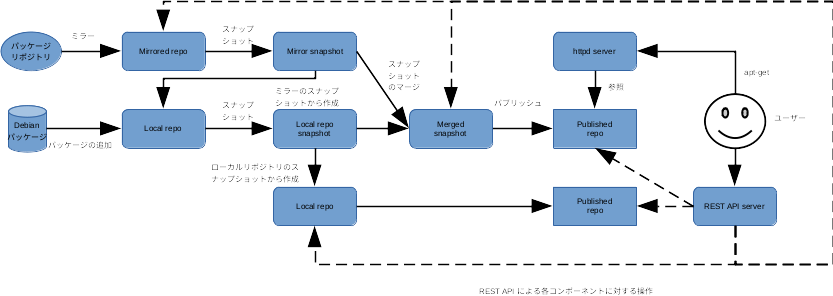
\includegraphics[width=1.0\hsize]{image202005/aptly-image00.png}

\begin{itemize}
\item ミラーリポジトリは他のパッケージリポジトリから作成します。
\item  ローカルパッケージはパッケージを追加するか、ローカルミラーから作成できます。
\item  作成したローカルミラーやローカルリポジトリはそのままではパッケージリポジトリとしては利用できず、パブリッシュ(公開)する必要があります。
\item  ローカルミラーやローカルリポジトリはスナップショットを作成できます。
\item  スナップショットからスナップショットも作成でき、スナップショット同士の依存関係もメタデータとして持ちます。
\item  スナップショット同士でマージできます。
\item  パプリッシュしたパッケージリポジトリは aptly で提供される httpサーバーを使用、またはその他httpサーバーを使って公開できます。
\end{itemize}

\subsubsection{aptly を使用する際に注意すること}

aptly ではパッケージリポジトリを公開する場合に、GnuPGによる署名が必要となります(必須ではなく、オプションで署名および
確認を無視できます)。aptly は一度ローカルにパッケージとメタ情報を保存し、
それらを組み合わせて、パッケージリポジトリに必要なメタデータ (Releaseファイルなど)を再構築
します。再構築したメタデータはフルミラーであっても内容が異なるため、正しくパッケージリポジトリ
を運用するにはこれらに GnuPG による署名が必要になります。
メタデータを含めたフルミラーを構築したい場合は archvsync (\url{https://salsa.debian.org/mirror-team/archvsync}) 
や apt-mirror パッケージを使うと良いでしょう。

またパッケージリポジトリの構築にはハードリンクを使います。よってハードリンクの制限が適用されることに注意
が必要です。Amazon S3 などのクラウドストレージにパッケージリポジトリをパブリッシュする際にはこの制限はありません。

以下からは、aptly に使い方について説明します。

\subsection{aptly のインストール}

aptlyは公式Debianパッケージとして提供されています。執筆時のDebianパッケージバージョンは 1.3.0+ds1-4 となっています。
以下のコマンドでインストールできます。

\begin{commandline}
$ sudo apt update
$ sudo apt install aptly
\end{commandline}

また Upstream のバージョンは 1.4.0 となっており、GnuPG 2.x へのサポート強化などが行われています。
最新バージョンを使いたい場合には、以下のようにアップストリーム が提供するリポジトリで提供されている
パッケージが利用できます。 ディストリビューション部が squeeze となっていますが、一つのディストリビューション
のみで提供されているので、気にしなくても良いです。

\begin{commandline}
$ wget -qO - https://www.aptly.info/pubkey.txt | sudo apt-key add -
$ sudo sh -c "echo deb http://repo.aptly.info/ squeeze main > /etc/apt/sources.list.d/aptly.list"
$ sudo apt update
$ sudo apt install aptly
\end{commandline}

\subsubsection{aptly の設定}

aptly の設定は \$HOME/.aptly.confに記載されています。
内容は aptly config コマンドの show サブコマンドで確認できます。
もちろん普段お使いのエディタ等で確認してもかまいません。

\begin{commandline}
$ aptly config show
{
    "rootDir": "/home/aptly/.aptly",
    "downloadConcurrency": 4,
    "downloadSpeedLimit": 0,
    "architectures": [],
    "dependencyFollowSuggests": false,
    "dependencyFollowRecommends": false,
    "dependencyFollowAllVariants": false,
    "dependencyFollowSource": false,
    "dependencyVerboseResolve": false,
    "gpgDisableSign": false,
    "gpgDisableVerify": false,
    "gpgProvider": "gpg",
    "downloadSourcePackages": false,
    "skipLegacyPool": true,
    "ppaDistributorID": "ubuntu",
    "ppaCodename": "",
    "skipContentsPublishing": false,
    "FileSystemPublishEndpoints": {},
    "S3PublishEndpoints": {},
    "SwiftPublishEndpoints": {}
}
\end{commandline}

詳細は省きますが、重要なのは rootDir の項目で、ここで指定されるディレクトリにaptly が管理する
パッケージのメタデータやローカルパッケージリポジトリ等が格納されます。
また Amazon S3や OpenStack Swift  へのアップロードを行う際には、S3PublishEndpointsやSwiftPublishEndpointsに対して
アクセスキー等を設定します。
各項目の詳細は Configuration (\url{https://www.aptly.info/doc/configuration/}) を確認してください。

\subsection{GnuPG 鍵の作成とパッケージリポジトリの署名確認必要な公開鍵のインポート}

aptly を使う前に、GnuPG鍵の作成と、パッケージミラー元のGnuPG公開鍵をインポートする
必要があります。
前述したように、正しくパッケージリポジトリを運用するにはGnuPGによる署名が必要なため、
GnuPG鍵を作成します。既にGnuPG鍵を持っている場合も、リポジトリ管理用に別途GnuPG鍵を
作成しておくとよいでしょう。GnuPG鍵の作成には以下のように実行します。

\begin{commandline}
$ gpg --gen-key

<中略>

本名: aptly
電子メール・アドレス: aptly@example.com
次のユーザIDを選択しました:
    "aptly <aptly@example.com>"

<中略>
公開鍵と秘密鍵を作成し、署名しました。

pub   rsa3072 2020-05-01 [SC] [有効期限: 2022-05-01]
      E67BDF3221F4CDFD47F4A3639A64752708B70EFA
uid                      aptly <aptly@example.com>
sub   rsa3072 2020-05-01 [E] [有効期限: 2022-05-01]
\end{commandline}

次にパッケージミラー元の GnuPG公開鍵をインポートします。
パッケージリポジトリのミラー元の情報を取得する際にミラー元の署名を確認する必要があるためです。
Debian のオフィシャルパッケージリポジトリを使う場合には以下のように実行します。

\begin{commandline}
$ sudo apt install debian-archive-keyring
$ gpg --no-default-keyring --keyring /usr/share/keyrings/debian-archive-keyring.gpg --export | \
        gpg --no-default-keyring --keyring trustedkeys.gpg --import
\end{commandline}

次に Debian で提供されているパッケージを使っている人は、GnuPG v2 で作成した鍵を v1 にコンバート
する必要があります。これは Debian のパッケージが GnuPG v1 に依存しているためです。
公開鍵 E67BDF3221F4CDFD47F4A3639A64752708B70EFA をコンバートし、GnuPG v1 にインポートする方法を
以下に示します。

\begin{commandline}
$ gpg --output gpg2_export_pub.gpg --armor --export E67BDF3221F4CDFD47F4A3639A64752708B70EFA
$ gpg --output gpg2_export_sec.gpg --armor --export-secret-key E67BDF3221F4CDFD47F4A3639A64752708B70EFA
$ gpg1 --import gpg2_export_pub.gpg
gpg: 鍵08B70EFA: 公開鍵"aptly <aptly@example.com>"をインポートしました
gpg:           処理数の合計: 1
gpg:             インポート: 1  (RSA: 1)
gpg: 最小の「ある程度の信用」3、最小の「全面的信用」1、PGP信用モデル
gpg: 深さ: 0  有効性:   1  署名:   0  信用: 0-, 0q, 0n, 0m, 0f, 1u
gpg: 次回の信用データベース検査は、2022-05-01です
$ gpg1 --import --allow-secret-key-import gpg2_export_sec.gpg
gpg: 鍵08B70EFA: 秘密鍵をインポートしました
gpg: 鍵08B70EFA:"aptly <aptly@example.com>"変更なし
gpg:           処理数の合計: 1
gpg:               変更なし: 1
gpg:       秘密鍵の読み込み: 1
gpg:     秘密鍵のインポート: 1
\end{commandline}

また作成するパッケージリポジトリにアクセスするマシンにパッケージリポジトリの公開鍵を登録することを
忘れないようにしましょう。公開鍵の出力方法と出力した公開鍵を登録する方法を以下に示します。

\begin{commandline}
$ gpg --export --armor > aptly.pub
\end{commandline}

\begin{commandline}
$ sudo apt-key add aptly.pub
\end{commandline}

\subsection{パッケージミラーリポジトリの作成}

ローカルにパッケージミラーリポジトリを作成する場合、 aptly mirror コマンドの create サブコマンドを使用します。
コマンドにローカルで利用する名前(name)、リポジトリのURL、ディストリビューション、コンポーネントを指定します。
例えば、

\begin{itemize}
	\item 名前: debian-buster
	\item リポジトリURL: http://deb.debian.org/debian/
	\item ディストリビューション: buster
	\item コンポーネント: main
	\item アーキテクチャ: すべて
\end{itemize}

上記のようなパッケージミラーリポジトリを作成する場合、以下のように実行します。
実行するとリポジトリが初期化されます。


\begin{commandline}
$ aptly mirror create debian-buster http://deb.debian.org/debian/ buster main
\end{commandline}

作成したパッケージミラーリポジトリの情報は list サブコマンドで
確認できます。

\begin{commandline}
$ aptly mirror list
List of mirrors:
 * [debian-buster]: http://deb.debian.org/debian/ buster

To get more information about mirror, run `aptly mirror show <name>`.
\end{commandline}

また詳細な情報が必要な場合は show サブコマンドで確認できます。

\begin{commandline}
$ aptly mirror show debian-buster
Name: debian-buster
Archive Root URL: http://deb.debian.org/debian/
Distribution: buster
Components: main
Architectures: amd64, arm64, armel, armhf, i386, mips, mips64el, mipsel, ppc64el, s390x
Download Sources: no
Download .udebs: no
Last update: never

Information from release file:
Acquire-By-Hash: yes
Architectures: amd64 arm64 armel armhf i386 mips mips64el mipsel ppc64el s390x
Changelogs: http://metadata.ftp-master.debian.org/changelogs/@CHANGEPATH@_changelog
Codename: buster
Components: main contrib non-free
Date: Sat, 09 May 2020 09:51:02 UTC
Description:  Debian 10.4 Released 09 May 2020

Label: Debian
Origin: Debian
Suite: stable
Version: 10.4
\end{commandline}

まだこの状態ではリポジトリのメタデータやパッケージがない状態のため、ミラー元から取得する必要があります。
取得するには update サブコマンドを実行します。
実行するとメタデータを取得し、パッケージのミラーを開始します。

\begin{commandline}
$ aptly mirror update debian-buster
\end{commandline}

上記では指定したディストリビューションのコンポーネントをすべてミラーします。
特定のアーキテクチャのみや、ミラーしたいパッケージを指定したい場合には、オプションを使うことで
制御できます。以下ではよく利用されるオプションを以下に示します。

\begin{itemize}
	\item アーキテクチャを指定する: -architectures
	\item パッケージをフィルターする: -filter
	\item フィルターで指定されたパッケージに依存するパッケージもミラーする: -filter-with-deps
	\item ソースパッケージもミラーする: -with-sources
\end{itemize}

アーキテクチャをamd64 と arm64、ミラーするパッケージを busybox、依存するパッケージとソースパッケージもミラーする場合
には以下のように実行します。

\begin{commandline}
$ aptly mirror create -architectures=amd64,arm64 -filter='busybox' \
    -filter-with-deps -with-sources busybox-mirror http://deb.debian.org/debian/ buster main
\end{commandline}

実行し、取得したパッケージは \$HOME/.aptly ディレクトリ以下に保存されます。
ファイルの配置は git リポジトリの git object のような配置になっています(sha265sum 値)。

\begin{commandline}
.aptly
├── db
│ ├── 000004.ldb
│ ├── 000007.ldb
│ ├── 000008.log
│ ├── CURRENT
│ ├── LOCK
│ ├── LOG
│ └── MANIFEST-000009
└── pool
    ├── 1b
    │ └── 00
    │     └── f7cef567645a7e695caf6c1ad395_gcc-8-base_8.3.0-6_amd64.deb
    ├── 1e
    │ └── 32
    │     └── ea742bddec4ed5a530ee2f423cdf_busybox_1.30.1-4_amd64.deb
<省略> 
\end{commandline}

作成したミラーで提供されるパッケージを確認するには aptly mirror コマンドの search サブコマンド使用します。
検索するミラー名と検索用のクエリーを指定し、実行します。以下に パッケージ名が busy\* 、アーキテクチャが
arm64 であるパッケージを検索するには以下のように実行します。検索用クエリーを指定しない場合は提供されるパ
ッケージが全て出力されます。

\begin{commandline}
$ aptly mirror search busybox-mirror 'Name (% busy*), $Architecture (arm64)'
busybox_1:1.30.1-4_arm64
busybox-static_1:1.30.1-4_arm64
\end{commandline}

\subsection{ローカルパッケージリポジトリの作成}

ローカルパッケージリポジトリは、独自で作成したパッケージをリポジトリで管理したい場合などに使用します。
まず管理するためのリポジトリを作成する必要があります。
リポジトリを作成するには、aptly repo コマンド のcreate サブコマンドに作成するリポジトリ名を指定して実行します。
このリポジトリ名は Debian パッケージで利用される ディストリビューション名 (unstable, buster など)
と紐付けられています。

\begin{commandline}
$ aptly repo create my-repo
\end{commandline}

またローカルリポジトリを作成する場合、スナップショットからも作成できます。

\begin{commandline}
$ aptly repo create my-repo from snapshot snapshot-name
\end{commandline}

\subsubsection{ローカルパッケージリポジトリへのパッケージの追加}

create サブコマンドで作成した段階では、ローカルパッケージリポジトリにまだパッケージが登録されていない状態なので、
パッケージを追加します。追加する方法は以下の方法があります。

\subsubsubsection{add サブコマンドを使ったパッケージの追加}

add サブコマンドは 特定のdebian バイナリパッケージ、またはdsc (Debian source packages control file)を元にソースパッケージを追加
したい場合に利用します。
パッケージを指定してローカルパッケージリポトリに追加したい場合は、add サブコマンドにパッケージファイルのパスを指定して実行します。

\begin{commandline}
$ aptly repo add my-repo pool/liblz4-1_1.9.2-2_amd64.deb
Loading packages...
[+] liblz4-1_1.9.2-2_amd64 added
\end{commandline}

またソースパッケージを追加したい場合には dsc ファイルを指定して実行します。

\begin{commandline}
$ aptly repo add my-repo pool/lz4_1.9.2-2.dsc
Loading packages...
[+] lz4_1.9.2-2_source added
\end{commandline}

特定のディレクトリにあるパッケージすべて追加したい場合には対象のディレクトリを指定すればよいです。

\begin{commandline}
$ aptly repo add my-repo pool
Loading packages...
[+] liblz4-1-dbgsym_1.9.2-2_amd64 added
[+] liblz4-1_1.9.2-2_amd64 added
[+] liblz4-dev_1.9.2-2_amd64 added
[+] liblz4-tool_1.9.2-2_all added
[+] lz4-dbgsym_1.9.2-2_amd64 added
[+] lz4_1.9.2-2_source added
[+] lz4_1.9.2-2_amd6 added
\end{commandline}

add コマンドを使った場合、ファイルのサイズやファイルハッシュ値の確認は行われないため注意が必要です。
より安全にパッケージをリポジトリに追加したい場合、次で説明する include サブコマンドを使います。

\subsubsubsection{include サブコマンドを使ったパッケージの追加}

ローカルパッケージリポジトリへのパッケージの追加には add サブコマンドの他にinclude サブコマンドも利用可能です。
add サブコマンドとの違いは処理の対象が .changes ファイルである事です。
.changes ファイルを指定して実行するには以下のように実行します。実行すると、.changes ファイルに記載されているパッケージ
が登録されます。特に指定しない場合、実行後にはパッケージファイル等は削除されてしまうので、削除したくない場合には
-no-remove-files オプションを指定する必要があります。
また.changes にGnuPGによる署名を行っておらず、署名の有無を無視したい場合には -accept-unsigned オプションを
指定する必要があります。

\begin{commandline}
Format: 1.8
Date: Tue, 12 Nov 2019 07:58:47 +0900
Source: lz4

<中略>

Checksums-Sha1:
 44348438b55dc32132df8039513a57c4c1cd87a5 1073 lz4_1.9.2-2.dsc
 3790bc3c9e6d4e26e5063855cf847f5af91d8420 12712 lz4_1.9.2-2.debian.tar.xz
 ce4d29ed984de507203d917e671c1894c9778e8c 323008 liblz4-1-dbgsym_1.9.2-2_amd64.deb
 aed6d84f4636d37cd94b90e9ce0320dee853eca6 57148 liblz4-1_1.9.2-2_amd64.deb
 018ef0f8bf34411b4b928072f5c1f2d1abf8103f 76752 liblz4-dev_1.9.2-2_amd64.deb
 bf32ee9eee03ef69d6b0526bed92dcc95af57883 5088 liblz4-tool_1.9.2-2_all.deb
 39f1aa1950030608ad528a4f4fe951b37e0e4956 410216 lz4-dbgsym_1.9.2-2_amd64.deb
 dec576464d1c5e4b2b69e59ab29208f4e6d741eb 6648 lz4_1.9.2-2_amd64.buildinfo
 689287ecea701b76f99c5d30040ca584bdc58fde 84076 lz4_1.9.2-2_amd64.deb

<省略>
\end{commandline}
 
\begin{commandline}
$ aptly repo include -repo my-repo pool/lz4_1.9.2-2_amd64.changes
Loading repository my-repo for changes file lz4_1.9.2-2_amd64.changes...
[+] liblz4-1-dbgsym_1.9.2-2_amd64 added
[+] liblz4-1_1.9.2-2_amd64 added
[+] liblz4-dev_1.9.2-2_amd64 added
[+] liblz4-tool_1.9.2-2_all added
[+] lz4-dbgsym_1.9.2-2_amd64 added
[+] lz4_1.9.2-2_source added
[+] lz4_1.9.2-2_amd64 added
\end{commandline}
%<!-- $ aptly repo include -repo my-repo -no-remove-files -accept-unsigned pool/lz4_1.9.2-2_amd64.changes -->

上記では実行する際に、-repo オプションでリポジトリ名を指定しています。
これは changelog で指定されているディストリビューション名(unstable など)がリポジトリ名と合致しない場合
にエラーになるためです。

またディレクトリを指定する場合には、.changes が格納されているデレクトリを指定します。

\begin{commandline}
$ aptly repo include -repo my-repo pool
Loading repository my-repo for changes file lz4_1.9.2-2_amd64.changes...
[+] liblz4-1-dbgsym_1.9.2-2_amd64 added
[+] liblz4-1_1.9.2-2_amd64 added
[+] liblz4-dev_1.9.2-2_amd64 added
[+] liblz4-tool_1.9.2-2_all added
[+] lz4-dbgsym_1.9.2-2_amd64 added
[+] lz4_1.9.2-2_source added
[+] lz4_1.9.2-2_amd64 added
\end{commandline}

指定したディレクトリに .changes ファイルがない場合や、.changes の内容が異なる場合には
処理されません。

\begin{commandline}
$ aptly repo include -repo my-repo -no-remove-files -accept-unsigned pool
[!] unable to process file lz4_1.9.2-2_amd64.changes: size mismatch: expected 12712 != obtained 12568 
[!] Some files were skipped due to errors:
  pool/lz4_1.9.2-2_amd64.changes
ERROR: some files failed to be added
\end{commandline}


% リポジトリのアップローダーを固定したい場合は**-uploaders-file=**を使う。
% uploaders のフォーマットは https://www.aptly.info/doc/aptly/repo/include/ に書いてある。

\subsubsubsection{ローカルミラーからの追加}

aptly mirror コマンドによって作成したローカルミラーで提供されているパッケージも
ローカルリポジトリに追加できます。この場合 import サブコマンドを利用します。

例えば、ローカルミラー busybox-mirror にある busybox で始まるパッケージを my-repo ローカル
リポジトリに追加する場合には以下のように実行します。

\begin{commandline}
$ aptly repo import busybox-mirror my-repo busybox
Loading packages...
[o] busybox_1:1.30.1-4_source imported
[o] busybox-static_1:1.30.1-4_amd64 imported
[o] busybox_1:1.30.1-4_arm64 imported
[o] busybox_1:1.30.1-4_amd64 imported
[o] busybox-static_1:1.30.1-4_arm64 imported
\end{commandline}

Package Queries(\url{https://www.aptly.info/doc/feature/query/})
にパッケージ名の指定方法等に関する説明があるので興味のある方は参照してください。

\subsubsection{ローカルパッケージリポジトリの削除}

ローカルパッケージリポジトリの情報を削除したい場合には、drop サブコマンドに削除したいリポジトリ名を指定します。

\begin{commandline}
$ aptly repo drop my-repo
\end{commandline}

\subsubsection{その他ローカルリポジトリに関する操作}

\begin{itemize}
\item repo list

  作成されたリポジトリのリストを出力します。

\item repo copy

  リポジトリにあるパッケージを指定したリポジトリにコピーします。
  コピー先のリポジトリは先に作成しておく必要がある点に注意が必要です。

\begin{commandline}
  $ aptlu repo create my-repo-next
  $ aptly repo copy my-repo my-repo-next 'Name (%lib*)'
  Loading packages...
  [o] liblz4-tool_1.9.2-2_all copied
  [o] liblz4-1_1.9.2-2_amd64 copied
  [o] liblz4-1-dbgsym_1.9.2-2_amd64 copied
  [o] liblz4-dev_1.9.2-2_amd64 copied
\end{commandline}

\item repo move

  リポジトリにあるパッケージを指定したリポジトリに移動します。
  コピー先のリポジトリは先に作成しておく必要がある点に注意が必要です。

\item repo remove

  指定したパッケージをリポジトリから削除します。

\item repo search

  リポジトリで提供されているパッケージを検索します。

\item repo edit

  リポジトリに関する情報を修正します。

\item repo rename

  リポジトリ名を変更します。

\end{itemize}

\subsection{スナップショット}

aptly mirror update コマンドを実行した場合、ミラー元のパッケージ情報等と完全に同期するため、
ミラー元で削除されたパッケージはローカルミラーでも削除され、更新されたパッケージも古いものは
残っていない状態になってしまいます。
またローカルパッケージリポジトリでも運用によっては上記と那じようなことが起こる可能性も
あります。このような事が起きても困らないようにするために、スナップショットを作成し、
パッケージの構成を維持できるよう管理します。

\subsubsection{スナップショットの作成と確認}

スナップショットを作成するには、aptly snapshot コマンドの create サブコマンドを使用します。
例えば、ローカルミラー buster-mirror のスナップショットを buster-mirror-2020512 として作成するには
以下のように実行します。

\begin{commandline}
$ aptly snapshot create buster-mirror-2020512 from mirror buster-mirror
\end{commandline}

スナッショットは ローカルリポジトリからも作成できます。
ローカルリポジトリ my-repo のスナップショットを my-repo-20200512 として作成するには以下のように
実行します。

\begin{commandline}
$ aptly snapshot create imy-repo-20200510 from repo my-repo
\end{commandline}

現在作成されているスナップショットを確認するには list サブコマンド、
スナップショットの情報を確認するにはは show サブコマンドを使います。

\begin{commandline}
$ aptly snapshot list
List of snapshots:
 * [busybox-buster-mirror-20200512]: Snapshot from mirror [busybox-buster-mirror]: http://deb.debian.org/debian/ buster
 * [my-repo-20200512]: Snapshot from local repo [my-repo]

To get more information about snapshot, run `aptly snapshot show <name>`.
$ aptly snapshot show my-repo-20200512
Name: my-repo-20200512
Created At: 2020-05-15 07:06:32 UTC
Description: Snapshot from local repo [my-repo]
Number of packages: 12
Sources:
  my-repo [local]
\end{commandline}

\subsubsection{スナップショットのマージ}

作成したスナップショットをマージし、新しいスナップショットを作成するには merge サブコマンドを使います。
作成したいスナップショット名にマージするスナップショットを指定します。

\begin{commandline}
$ aptly snapshot merge my-product-release-20200512 my-repo-20200512 busybox-buster-mirror-20200512

Snapshot my-product-release-20200512 successfully created.
You can run 'aptly publish snapshot my-product-release-20200512' to publish snapshot as Debian repository.
$ aptly snapshot list
List of snapshots:
 * [busybox-buster-mirror-20200512]: Snapshot from mirror [busybox-buster-mirror]: http://deb.debian.org/debian/ buster
 * [my-product-release-20200512]: Merged from sources: 'my-repo-20200512', 'busybox-buster-mirror-20200512'
 * [my-repo-20200512]: Snapshot from local repo [my-repo]

To get more information about snapshot, run `aptly snapshot show <name>`.

$ aptly snapshot show my-product-release-20200512
Name: my-product-release-20200512
Created At: 2020-05-15 07:20:35 UTC
Description: Merged from sources: 'my-repo-20200512', 'busybox-buster-mirror-20200512'
Number of packages: 15
Sources:
  my-repo-20200512 [snapshot]
  busybox-buster-mirror-20200512 [snapshot]
\end{commandline}

\subsubsection{スナップショットの検証}

スナップショットの状態によってはパッケージの依存関係が維持できてない場合があります。
これはパッケージの追加し忘れや、ローカルミラーリポジトリを
構築した際に -filter-with-deps オプションを付けていなかったことなどが原因となります。
このような状態を確認するために、スナップショット内容を検証するサブコマンド verify が
用意されています。
以下では、-filter-with-deps を付けずに busyboxから始まるパッケージのミラーを作成し、
そのスナップショットを検証した結果です。このスナップショットでは libc6 (>= 2.28) が
不足していることがわかります。

\begin{commandline}
$ aptly mirror create -architectures=amd64 -filter='busybox' \
    busybox-buster-mirror-without-dep http://deb.debian.org/debian/ buster main
$ aptly mirror update busybox-buster-mirror-without-dep
$ aptly snapshot create busybox-buster-mirror-without-dep-v1 from mirror busybox-buster-mirror-without-dep
$ aptly snapshot verify busybox-buster-mirror-without-dep-v1
Loading packages...
Verifying...
Missing dependencies (1):
  libc6 (>= 2.28) [amd64]
\end{commandline}

このような場合、足りないパッケージを提供するリモートパッケージリポジトリを apt-line に追加するなどで対応できますが、
このリモートパッケージリポジトリの内容が変更される可能性も考えられます。根本的に問題を回避するためには、同じスナップショット
内で提供できるようにしたほうがよいでしょう。
スナップショットのベースとなったミラーを -filter-with-deps 付加した後更新し、再度スナップショットを作成するか、
他のスナップショットで必要とするパッケージが提供されているなら、次で説明する pull サブコマンドを使って、他のスナップショットから
パッケージを取り込むこともできます。

\begin{commandline}
$ aptly mirror edit -filter-with-deps busybox-buster-mirror-without-dep
$ aptly mirror show busybox-buster-mirror | grep '^Filter With Deps'
Filter With Deps: yes
$ aptly mirror update busybox-buster-mirror
\end{commandline}

\subsubsubsection{他のスナップショットからパッケージを取り込み、新しいスナップショットを作成する}

既存のスナップショットに、他のスナップショットで提供されるパッケージを取り込み、新しいスナップショット
を作成するには、pull サブコマンドを使います。
ベースとするスナップショット busybox-buster-mirror-without-dep-v1 に スナップショット libc-dev-mirror-20200512 で
提供される libc6 パッケージを取り込み、スナップショット busybox-buster-mirror-v1 を作成するには、以下のように実行
します。

\begin{commandline}
$ aptly snapshot pull busybox-buster-mirror-without-dep-v1 libc-dev-mirror-20200512 busybox-buster-mirror-v1 libc6
Dependencies would be pulled into snapshot:
    [busybox-buster-mirror-without-dep-v1]: Snapshot from mirror [busybox-buster-mirror-without-dep]: \
	http://deb.debian.org/debian/ buster
from snapshot:
    [libc-dev-mirror-20200512]: Snapshot from mirror [libc-dev-mirror]: http://deb.debian.org/debian/ buster
and result would be saved as new snapshot busybox-buster-mirror-v1.
Loading packages (8)...
Building indexes...
[+] gcc-8-base_8.3.0-6_amd64 added
[+] libc6_2.28-10_amd64 added
[+] libgcc1_1:8.3.0-6_amd64 added

Snapshot busybox-buster-mirror-v1 successfully created.
You can run 'aptly publish snapshot busybox-buster-mirror-v1' to publish snapshot as Debian repository.
\end{commandline}

新しく作成されたスナップショット busybox-buster-mirror-v1 を確認すると、libc6 パッケージとlibc6に依存するパッケージ
が取り込まれ、verify サブオプションの結果も問題ないことがわかります。

\begin{commandline}
$ aptly snapshot show -with-packages busybox-buster-mirror-v1
Name: busybox-buster-mirror-v1
Created At: 2020-05-15 18:13:45 UTC
Description: Pulled into 'busybox-buster-mirror-without-dep-v1' with 'libc-dev-mirror-20200512' as source, \
	pull request was: 'libc6'
Number of packages: 5
Sources:
  busybox-buster-mirror-without-dep-v1 [snapshot]
  libc-dev-mirror-20200512 [snapshot]
Packages:
  busybox_1:1.30.1-4_amd64
  busybox-static_1:1.30.1-4_amd64
  gcc-8-base_8.3.0-6_amd64
  libc6_2.28-10_amd64
  libgcc1_1:8.3.0-6_amd64
$ aptly snapshot verify busybox-buster-mirror-v1
Loading packages...
Verifying...
All dependencies are satisfied.
\end{commandline}

\subsubsubsection{スナップショットの削除}

スナップショットを削除する場合、drop サブコマンドを使用します。
削除するスナップショットが他のスナップショットでマージされている場合には削除されません。
-force オプションで強制的に削除もできますが、リポジトリの整合性がなくなる可能性があるので、
マージ先のスナップショットを削除してから、削除するようにします。
下記の実行例では、スナップショット my-repo-20200512 は スナップショット my-product-release-20200512
に依存されているため、削除できません。
\begin{commandline}
$ aptly snapshot drop my-repo-20200512
Snapshot `my-repo-20200512` was used as a source in following snapshots:
 * [my-product-release-20200512]: Merged from sources: 'my-repo-20200512', 'busybox-buster-mirror-20200512'
ERROR: won't delete snapshot that was used as source for other snapshots, use -force to override
\end{commandline}

もしスナップショット my-repo-20200512 を削除したい場合には、依存されている my-product-release-20200512を
先に削除する必要があります。

\begin{commandline}
$ aptly snapshot drop my-product-release-20200512
Snapshot `my-product-release-20200512` has been dropped.
$ aptly snapshot drop my-repo-20200512
Snapshot `my-repo-20200512` has been dropped.
\end{commandline}

\subsubsubsection{スナップショットに関する他の機能}
\begin{itemize}
\item diff

  スナップショット間の差分を出力します。

\item search 

  指定したスナップショットで提供されているパッケージを検索します。

\item rename

  スナップショット名を変更します。

\end{itemize}

\subsection{リポジトリの公開(パブリッシュ)}

これまでローカルミラーやローカルリポジトリ、スナップショットについて説明してきましたが、
これまでの状態ではまだ apt-line として参照できるパッケージリポジトリにはなっていないため、
apt コマンド等でパッケージのダウロードやインストールはできません。publish コマンドを用いて
パッケージリポジトリを公開する必要があります。

公開するパッケージリポジトリはスナップショットとローカルパッケージリポジトリから作成できますが、
後者は推奨されません。この理由として、ローカルパッケージリポジトリはスナップショットとは異なり、
内容が変更される可能性があるためです。以下ではスナップショットをパッケージリポジトリとして
公開する方法を説明します。

\subsubsection{スナップショットからパッケージリポジトリを作成する}

スナップショット my-product-release-20200512 をパッケージリポジトリとして公開する場合、
snapshot サブコマンドにスナップショット名を指定して実行します。実行すると GnuPG 署名
するにパスフレーズを要求されます。

\begin{commandline}
$ aptly publish snapshot my-product-release-20200512 
Loading packages...
Generating metadata files and linking package files...
Finalizing metadata files...
Signing file 'Release' with gpg, please enter your passphrase when prompted:

次のユーザの秘密鍵のロックを解除するには
パスフレーズがいります:"aptly <aptly@example.com>"
3072ビットRSA鍵, ID 08B70EFA作成日付は2020-05-10

Clearsigning file 'Release' with gpg, please enter your passphrase when prompted:

次のユーザの秘密鍵のロックを解除するには
パスフレーズがいります:"aptly <aptly@example.com>"
3072ビットRSA鍵, ID 08B70EFA作成日付は2020-05-10

Snapshot my-product-release-20200512 has been successfully published.
Please setup your webserver to serve directory '/home/aptly/.aptly/public' with autoindexing.
Now you can add following line to apt sources:
  deb http://your-server/ buster main
  deb-src http://your-server/ buster main
Don't forget to add your GPG key to apt with apt-key.

You can also use `aptly serve` to publish your repositories over HTTP quickly.
\end{commandline}
 
パッケージリポジトリは \$(HOME)/.aptly/public 以下に作成されます。
対象ディレクトリをapt-line で参照できるように設定すると、apt コマンド等からパッケージを取得できる
ようになります。
また上記出力にあるように apt-line で設定する内容をディストリビューション名が buster になっています。
これは スナップショット my-product-release-20200512 のベースが Debian ミラーの buster ディストリ
ビューションだったためです。ディストリビューション名を変更したい場合には、-distribution オプションを
使います。

\begin{commandline}
$ aptly publish snapshot -distribution="my-product" my-product-release-20200512 
<省略>

Now you can add following line to apt sources:
  deb http://your-server/ my-product main
  deb-src http://your-server/ my-product main
\end{commandline}

\subsubsection{パッケージリポジトリの更新}

パッケージリポジトリ内容を、新しく作成したスナップショットに更新したい場合、switch サブコマンドを使います。
以下では、zlib1g パッケージを含んだスナップショットをマージした スナップショット my-product-release-20200513
に更新しています。

\begin{commandline}
$ aptly mirror drop zlib-buster-mirror
$ aptly mirror create -architectures=amd64 -filter='zlib1g' -filter-with-deps zlib-buster-mirror \
	http://deb.debian.org/debian/ buster main
$ aptly mirror update zlib-buster-mirror
$ aptly snapshot create zlib-buster-mirror-20200512 from mirror zlib-buster-mirror
$ aptly snapshot merge my-product-release-20200513 my-repo-20200512 busybox-buster-mirror-20200512 zlib-buster-mirror-20200512
$ aptly snapshot diff my-product-release-20200512 my-product-release-20200513
  Arch   | Package | Version in A | Version in B
+ amd64  | zlib1g  | -            | 1:1.2.11.dfsg-1
$ aptly publish switch my-product my-product-release-20200513
Loading packages...
Generating metadata files and linking package files...
Finalizing metadata files...
Signing file 'Release' with gpg, please enter your passphrase when prompted:

<省略>
\end{commandline}

\subsubsection{公開されているパッケージリポジトリの確認}

公開されているパッケージリポジトリを確認するには list サブコマンドを使います。
これにより公開されているパッケージリポジトリがどのスナップショット・ローカルパッケージリポジトリに依存しているのか
確認できます。

\begin{commandline}
$ aptly publish list
Published repositories:
  * ./buster [amd64, source] publishes {main: [my-product-release-20200512]: Merged from sources: \
	'my-repo-20200512', 'busybox-buster-mirror-20200512'}
  * ./my-product [amd64, source] publishes {main: [my-product-release-20200513]: Merged from sources: \
	'my-repo-20200512', 'busybox-buster-mirror-20200512', 'zlib-buster-mirror-20200512'}
\end{commandline}

パッケージリポジトリでサポートしているアーキテクチャなども確認したい場合には show サブコマンドを使います。

\begin{commandline}
$ aptly publish show my-product
Prefix: .
Distribution: my-product
Architectures: amd64 source
Sources:
  main: my-product-release-20200513 [snapshot]
\end{commandline}

\subsubsection{パッケージリポジトリの削除}

パッケージリポジトリを削除するには drop サブコマンドを使います。
実行するとパッケージリポジトリ出力先ディレクトリも削除されます。

\begin{commandline}
$ aptly publish drop buster
$ aptly publish list
Published repositories:
  * ./my-product [amd64, source] publishes {main: [my-product-release-20200513]: Merged from sources: \
	'my-repo-20200512', 'busybox-buster-mirror-20200512', 'zlib-buster-mirror-20200512'}
\end{commandline}

\subsubsection{パッケージリポジトリへのアクセス}

パブリッシュしたパッケージリポジトリで提供されるパッケージを利用するには、以下の3つの方法があります。

\begin{enumerate}
	\item File プロトコルを使用して、.aptly/public/ をapt-line に追加する。
	\item aptly で提供される http サーバーを立ち上げ、http 経由で取得する。
	\item 別途 HTTP サーバーを立ち上げ、.aptly/public/を参照するよう設定し、http 経由で取得する。
\end{enumerate}

各々の方法を以下に説明します。

\subsubsubsection{File プロトコルを使う}

File プロトコルを使う場合には、apt-line に パッケージリポジトリを指定します。
この場合、パッケージリポジトリを提供しているマシン以外からはアクセスできない点に注意が必要です。

\begin{commandline}
$ sudo sh -c "echo deb file:///home/aptly/.aptly/public/ my-product main" >> /etc/apt/sources.list.d/my-product.list
$ sudo apt update
\end{commandline}

\subsubsubsection{aptly で提供される http サーバー使う}

aptly で提供される http サーバーを使うには、aptly serve コマンドを使います。
実行すると パッケージリポジトリへ8080番ポート経由でアクセスできるようになります。

\begin{commandline}
$ aptly serve
Serving published repositories, recommended apt sources list:

# ./my-product [amd64, source] publishes {main: [my-product-release-20200513]: Merged from sources: 'my-repo-20200512', \
	'busybox-buster-mirror-20200512', 'zlib-buster-mirror-20200512'}
deb http://ryzen7:8080/ my-product main
deb-src http://ryzen7:8080/ my-product main

Starting web server at: :8080 (press Ctrl+C to quit)...
\end{commandline}

その後アクセスするマシンに apt-line を追加することで、パッケージリポジトリにアクセスできるようになります。
\begin{commandline}
$ sudo sh -c "echo deb http://ryzen7:8080/ my-product main" > /etc/apt/sources.list.d/my-product.list
$ sudo apt update
\end{commandline}

アクセスするためのポートやホスト名を指定したい場合には -listen オプションを使います。
ローカルループバックアドレス 127.0.0.1 の 8888番ポートとして起動したい場合には以下のように実行します。
\begin{commandline}
$ aptly serv -listen=127.0.0.1:8888
\end{commandline}

\subsubsubsection{別途 パッケージリポジトリ用 http サーバーを立ち上げる}

nginx を例に http サーバーの設定方法を説明します。
nginx をインストールし、/etc/nginx/sites-available/apt を作成します。

\begin{commandline}
$ sudo apt-get install nginx
$ sudo vi /etc/nginx/sites-available/apt
\end{commandline}

\begin{commandline}
server {
    listen 80; 
    listen [::]:80;
 
    server_name aptly.exaple.com;
    root /var/www-apt;
    allow all;
    autoindex on; 
 
    # Full access for everybody for the stable debian repo
    location /public {
        root /home/aptly/.aptly;
        allow all;
    }
 
    # Allow access to the top level to be able to download the GPG key 
    location / { 
        allow all;
    }
}
\end{commandline}

/etc/nginx/sites-enabled/apt にシンボリックリンクを作成し、nginx を再起動します。
\begin{commandline}
$ sudo ln -s /etc/nginx/sites-available/apt /etc/nginx/sites-enabled/apt
$ sudo systemctl restart nginx
\end{commandline}

その後アクセスするマシンに apt-line を追加することで、パッケージリポジトリにアクセスできるようになります。
\begin{commandline}
$ sudo sh -c "echo deb http://ryzen/public/ my-product main" > /etc/apt/sources.list.d/my-product.list
$ sudo apt update
\end{commandline}

\subsection{REST API}

aptly は REST API が提供されており、API 用サーバーを立ち上げることで利用できるようになります。
API サーバーの起動は aptly api コマンドの serve サブオプションを実行します。

\begin{commandline}
$ aptly api serve
Starting web server at: :8080 (press Ctrl+C to quit)...
[GIN-debug] [WARNING] Now Gin requires Go 1.6 or later and Go 1.7 will be required soon.
...
\end{commandline}

起動した後は、サーバーに対して API を実行できるようになります。
repo、snapshot、publish、package、graph に関するAPIが提供されており、
mirror や db に対する API はまだ提供されていません。
API の詳細は Web サイトのAPI (\url{https://www.aptly.info/doc/api/})に記載されています。
ここでは API の使い方をいくつか紹介します。

\begin{itemize}
  \item ローカルパッケージリポジトリで提供されているパッケージ一覧を取得する。

\begin{commandline}
$ curl http://localhost:8080/api/repos/my-repo/packages
["Pamd64 lz4 1.9.2-2 76bbfff77a824848","Pamd64 lz4-dbgsym 1.9.2-2 e71a271edd2c351","Psource lz4 1.9.2-2 91576aff056e5141",\
	"Pall liblz4-tool 1.9.2-2 8db5a921d2f58813","Pamd64 liblz4-1 1.9.2-2 30f3b73d9c877f6b",\
	"Pamd64 liblz4-1-dbgsym 1.9.2-2 7a9c4cd5844174f8","Pamd64 liblz4-dev 1.9.2-2 9f649d10440c4c7f"]
\end{commandline}

 \item スナップショットに関する情報を取得する。

\begin{commandline}
$ curl http://localhost:8080/api/snapshots
[{"Name":"busybox-buster-mirror-20200512","CreatedAt":"2020-05-15T19:29:25.376281727Z",\
	"Description":"Snapshot from mirror [busybox-buster-mirror]: http://deb.debian.org/debian/ buster","Origin":"Debian",\
	"NotAutomatic":"","ButAutomaticUpgrades":""},
	{"Name":"busybox-buster-mirror-without-dep-v1","CreatedAt":"2020-05-15T18:09:04.530501686Z",\
	"Description":"Snapshot from mirror [busybox-buster-mirror-without-dep]: http://deb.debian.org/debian/ buster",
	"Origin":"Debian","NotAutomatic":"","ButAutomaticUpgrades":""},
	{"Name":"my-product-release-20200512","CreatedAt":"2020-05-15T21:51:09.772154566Z",\
	"Description":"Merged from sources: 'my-repo-20200512', 'busybox-buster-mirror-20200512'","Origin":"",
	"NotAutomatic":"", "ButAutomaticUpgrades":""}, \
	{"Name":"my-product-release-20200513","CreatedAt":"2020-05-15T19:38:33.373419548Z", \
	"Description":"Merged from sources: 'my-repo-20200512', 'busybox-buster-mirror-20200512', 
	'zlib-buster-mirror-20200512'", "Origin":"","NotAutomatic":"","ButAutomaticUpgrades":""}, \
	{"Name":"my-repo-2* Connection #0 to host localhost left intact 0200512","CreatedAt":"2020-05-15T19:29:26.185504839Z", \
	"Description":"Snapshot from local repo [my-repo]","Origin":"","NotAutomatic":"","ButAutomaticUpgrades":""}, \
	{"Name":"zlib-buster-mirror-20200512","CreatedAt":"2020-05-15T19:29:25.510882855Z", \
	"Description":"Snapshot from mirror [zlib-buster-mirror]: http://deb.debian.org/debian/ buster","Origin":"Debian"," \
	NotAutomatic":"","ButAutomaticUpgrades":""}]
\end{commandline}

 \item ローカルパッケージリポジトリ my-repo のスナップショット を my-repo-devel として作成する

\begin{commandline}
$ curl -X POST -H 'Content-Type: application/json' --data '{"Name":"my-repo-devel"}' \
	http://localhost:8080/api/repos/my-repo/snapshots
{"Name":"my-repo-devel","CreatedAt":"2020-05-16T09:44:46.985707235+09:00", \
	"Description":"Snapshot from local repo [my-repo]","Origin":"","NotAutomatic":"","ButAutomaticUpgrades":""}
\end{commandline}

\end{itemize}

\subsubsection{REST API を扱うソフトウェア}

REST API は直接扱いづらいため、Python や Ruby などのプログラミング言語で操作したいと思う人がほとんどだと思います。
aptly を扱うツールやAPIラッパーを紹介します。

\begin{itemize}
  \item Python
    \begin{itemize}
    \item aptly-api-client / \url{https://github.com/gopythongo/aptly-api-client}
    \item python-aptly / \url{https://github.com/tcpcloud/python-aptly}
    \item, pyaptly / \url{https://github.com/adfinis-sygroup/pyaptly}
    \end{itemize}

  \item Ruby
    \begin{itemize}
    \item aptly\_cli / \url{https://github.com/sepulworld/aptly_cli}
    \item aptly-simple / \url{https://github.com/serge-name/aptly-simple}
    \item aptlier / \url{https://github.com/3ofcoins/aptlier}
    \end{itemize}

  \item shell
    \begin{itemize}
    \item  nitrux-repository-util / \url{(https://github.com/Nitrux/nitrux-repository-util}
    \end{itemize}
\end{itemize}

\subsection{まとめ}

Debianパッケージリポジトリの統合ツールである aptly の使い方を紹介しました。
APIの機能はまだ足りてない部分も多く、使いづらいところはありますが、
dpkg-dev や apt-ftparchive 使いながらCI/CD環境を構築されている方はもちろん、
会社のインフラ整備やDebian/Ubuntuをつかった製品開発をされている方やDebianパッケージ
メンテナにも有用なツールです。これを機会に aptly へのきりかえを検討してみませんか。

% 冊子にするために、4の倍数にする必要がある。
% そのための調整
\dancersection{メモ}{}
\mbox{}\newpage
\mbox{}\newpage
\mbox{}\newpage

\vspace*{15cm}
\hrule
\vspace{2mm}

\includegraphics[width=2cm]{image200502/openlogo-nd.eps}
\noindent \Large \bf Debian 勉強会資料\\
\noindent \normalfont \debmtgyear{}年\debmtgmonth{}月\debmtgdate{}日 \hspace{5mm}  初版第1刷発行\\
\noindent \normalfont 東京エリア Debian 勉強会 (編集・印刷・発行)\\
\hrule
\end{document}
